\documentclass{standalone}
\usepackage{tikz}
\usetikzlibrary{patterns, positioning}


\begin{document}
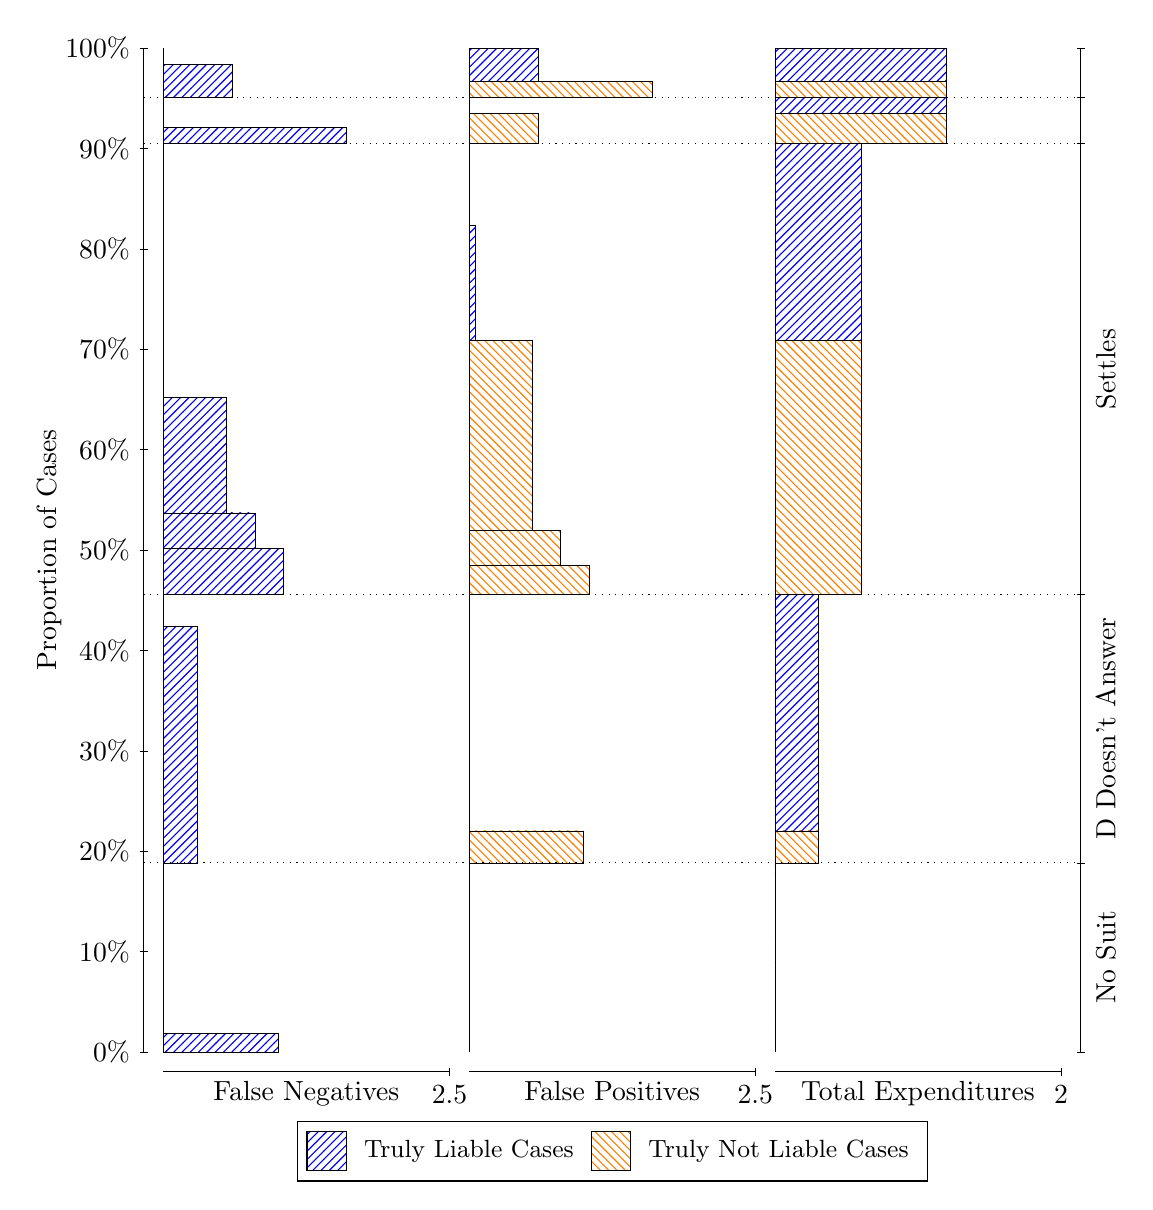
\begin{tikzpicture}
\draw[black, very thin] (1.5,1.75) -- (1.5,14.5);
\node[rotate=90, text=black, anchor=center] at (0.3, 8.125) {Proportion of Cases};
\draw[black, very thin] (1.45,1.75) -- (1.55,1.75);
\node[text=black, anchor=east] at (1.45, 1.75) {0\%};
\draw[black, very thin] (1.45,3.025) -- (1.55,3.025);
\node[text=black, anchor=east] at (1.45, 3.025) {10\%};
\draw[black, very thin] (1.45,4.3) -- (1.55,4.3);
\node[text=black, anchor=east] at (1.45, 4.3) {20\%};
\draw[black, very thin] (1.45,5.575) -- (1.55,5.575);
\node[text=black, anchor=east] at (1.45, 5.575) {30\%};
\draw[black, very thin] (1.45,6.85) -- (1.55,6.85);
\node[text=black, anchor=east] at (1.45, 6.85) {40\%};
\draw[black, very thin] (1.45,8.125) -- (1.55,8.125);
\node[text=black, anchor=east] at (1.45, 8.125) {50\%};
\draw[black, very thin] (1.45,9.4) -- (1.55,9.4);
\node[text=black, anchor=east] at (1.45, 9.4) {60\%};
\draw[black, very thin] (1.45,10.675) -- (1.55,10.675);
\node[text=black, anchor=east] at (1.45, 10.675) {70\%};
\draw[black, very thin] (1.45,11.95) -- (1.55,11.95);
\node[text=black, anchor=east] at (1.45, 11.95) {80\%};
\draw[black, very thin] (1.45,13.225) -- (1.55,13.225);
\node[text=black, anchor=east] at (1.45, 13.225) {90\%};
\draw[black, very thin] (1.45,14.5) -- (1.55,14.5);
\node[text=black, anchor=east] at (1.45, 14.5) {100\%};

\draw[black, very thin] (13.4,1.75) -- (13.4,14.5);
\draw[black, very thin] (13.35,1.75) -- (13.45,1.75);
\node[anchor=west] at (13.35, 1.75) {};
\draw[black, very thin] (13.35,4.1507) -- (13.45,4.1507);
\node[anchor=west] at (13.35, 4.1507) {};
\draw[black, very thin] (13.35,7.5599) -- (13.45,7.5599);
\node[anchor=west] at (13.35, 7.5599) {};
\draw[black, very thin] (13.35,13.286) -- (13.45,13.286);
\node[anchor=west] at (13.35, 13.286) {};
\draw[black, very thin] (13.35,13.87) -- (13.45,13.87);
\node[anchor=west] at (13.35, 13.87) {};
\draw[black, very thin] (13.35,14.5) -- (13.45,14.5);
\node[anchor=west] at (13.35, 14.5) {};

\draw[black, very thin, pattern color=blue, pattern=north east lines] (1.75,1.75) rectangle (3.2033,1.991);
\draw[black, very thin, pattern color=orange, pattern=north west lines] (1.75,1.991) rectangle (1.75,4.1507);
\draw[black, very thin, pattern color=blue, pattern=north east lines] (1.75,4.1507) rectangle (2.186,7.154);
\draw[black, very thin, pattern color=orange, pattern=north west lines] (1.75,7.154) rectangle (1.75,7.5599);
\draw[black, very thin, pattern color=blue, pattern=north east lines] (1.75,7.5599) rectangle (3.276,8.1471);
\draw[black, very thin, pattern color=blue, pattern=north east lines] (1.75,8.1471) rectangle (2.9127,8.5952);
\draw[black, very thin, pattern color=blue, pattern=north east lines] (1.75,8.5952) rectangle (2.5493,10.06);
\draw[black, very thin, pattern color=orange, pattern=north west lines] (1.75,10.06) rectangle (1.75,13.286);
\draw[black, very thin, pattern color=blue, pattern=north east lines] (1.75,13.286) rectangle (4.0753,13.49);
\draw[black, very thin, pattern color=orange, pattern=north west lines] (1.75,13.49) rectangle (1.75,13.87);
\draw[black, very thin, pattern color=blue, pattern=north east lines] (1.75,13.87) rectangle (2.622,14.296);
\draw[black, very thin, pattern color=orange, pattern=north west lines] (1.75,14.296) rectangle (1.75,14.5);
\draw[black, very thin, pattern color=orange, pattern=north west lines] (5.6333,1.75) rectangle (5.6333,3.9097);
\draw[black, very thin, pattern color=blue, pattern=north east lines] (5.6333,3.9097) rectangle (5.6333,4.1507);
\draw[black, very thin, pattern color=orange, pattern=north west lines] (5.6333,4.1507) rectangle (7.0867,4.5566);
\draw[black, very thin, pattern color=blue, pattern=north east lines] (5.6333,4.5566) rectangle (5.6333,7.5599);
\draw[black, very thin, pattern color=orange, pattern=north west lines] (5.6333,7.5599) rectangle (7.1593,7.926);
\draw[black, very thin, pattern color=orange, pattern=north west lines] (5.6333,7.926) rectangle (6.796,8.3761);
\draw[black, very thin, pattern color=orange, pattern=north west lines] (5.6333,8.3761) rectangle (6.4327,10.786);
\draw[black, very thin, pattern color=blue, pattern=north east lines] (5.6333,10.786) rectangle (5.706,12.251);
\draw[black, very thin, pattern color=blue, pattern=north east lines] (5.6333,12.251) rectangle (5.6333,13.286);
\draw[black, very thin, pattern color=orange, pattern=north west lines] (5.6333,13.286) rectangle (6.5053,13.666);
\draw[black, very thin, pattern color=blue, pattern=north east lines] (5.6333,13.666) rectangle (5.6333,13.87);
\draw[black, very thin, pattern color=orange, pattern=north west lines] (5.6333,13.87) rectangle (7.9587,14.073);
\draw[black, very thin, pattern color=blue, pattern=north east lines] (5.6333,14.073) rectangle (6.5053,14.5);
\draw[black, very thin, pattern color=orange, pattern=north west lines] (9.5167,1.75) rectangle (9.5167,3.9097);
\draw[black, very thin, pattern color=blue, pattern=north east lines] (9.5167,3.9097) rectangle (9.5167,4.1507);
\draw[black, very thin, pattern color=orange, pattern=north west lines] (9.5167,4.1507) rectangle (10.062,4.5566);
\draw[black, very thin, pattern color=blue, pattern=north east lines] (9.5167,4.5566) rectangle (10.062,7.5599);
\draw[black, very thin, pattern color=orange, pattern=north west lines] (9.5167,7.5599) rectangle (10.607,10.786);
\draw[black, very thin, pattern color=blue, pattern=north east lines] (9.5167,10.786) rectangle (10.607,13.286);
\draw[black, very thin, pattern color=orange, pattern=north west lines] (9.5167,13.286) rectangle (11.697,13.666);
\draw[black, very thin, pattern color=blue, pattern=north east lines] (9.5167,13.666) rectangle (11.697,13.87);
\draw[black, very thin, pattern color=orange, pattern=north west lines] (9.5167,13.87) rectangle (11.697,14.073);
\draw[black, very thin, pattern color=blue, pattern=north east lines] (9.5167,14.073) rectangle (11.697,14.5);
\draw[black, dotted] (1.5,4.1507) -- (13.4,4.1507);
\draw[black, dotted] (1.5,7.5599) -- (13.4,7.5599);
\draw[black, dotted] (1.5,13.286) -- (13.4,13.286);
\draw[black, dotted] (1.5,13.87) -- (13.4,13.87);
\draw[black, very thin] (1.75,1.5) -- (5.3833,1.5);
\node[text=black, anchor=north] at (3.5667, 1.5) {False Negatives};
\draw[black, very thin] (5.3833,1.45) -- (5.3833,1.55);
\node[text=black, anchor=north] at (5.3833, 1.45) {2.5};

\draw[black, very thin] (5.6333,1.5) -- (9.2667,1.5);
\node[text=black, anchor=north] at (7.45, 1.5) {False Positives};
\draw[black, very thin] (9.2667,1.45) -- (9.2667,1.55);
\node[text=black, anchor=north] at (9.2667, 1.45) {2.5};

\draw[black, very thin] (9.5167,1.5) -- (13.15,1.5);
\node[text=black, anchor=north] at (11.333, 1.5) {Total Expenditures};
\draw[black, very thin] (13.15,1.45) -- (13.15,1.55);
\node[text=black, anchor=north] at (13.15, 1.45) {2};

\node[text=black, centered, rotate=90] at (13.72, 2.9503) {No Suit};
\node[text=black, centered, rotate=90] at (13.72, 5.8553) {D Doesn't Answer};
\node[text=black, centered, rotate=90] at (13.72, 10.423) {Settles};



\draw (7.449999999999999,1.5) node[draw=none] (baseCoordinate) {};
\begin{scope}[align=center]
        \matrix[scale=0.5, draw=black, below=0.5cm of baseCoordinate, nodes={draw}, column sep=0.1cm]{
            \node[rectangle, draw, minimum width=0.5cm, minimum height=0.5cm, pattern color=blue, pattern=north east lines] {}; &
            \node[draw=none, font=\small, text=black] (B) {Truly Liable Cases}; &
            \node[rectangle, draw, minimum width=0.5cm, minimum height=0.5cm, pattern color=orange, pattern=north west lines] {}; &
            \node[draw=none, font=\small, text=black] (B) {Truly Not Liable Cases}; \\
            };
\end{scope}

\end{tikzpicture}
\end{document}